% Informe final — Minería de Datos 2026-I (UNMSM-FISI)
% Compilar: pdflatex informe.tex (dos pasadas para referencias)
\documentclass[11pt,a4paper]{article}

\usepackage[utf8]{inputenc}
\usepackage[T1]{fontenc}
\usepackage[spanish,es-tabla,es-nolists]{babel}
\decimalpoint  % decimales con punto en todo el documento (coherente con dashboard y notebooks)
\usepackage{mathptmx}
\usepackage[margin=2.5cm]{geometry}
\usepackage{graphicx}
\usepackage{booktabs}
\usepackage[table]{xcolor}
\usepackage{caption}
\usepackage[colorlinks=true,linkcolor=black,urlcolor=blue!50!black]{hyperref}

\captionsetup{font=small,labelfont=bf}
\setlength{\parskip}{4pt}

\begin{document}

% =====================================================================
% CARATULA - PAGINA UNICA EN UNA COLUMNA
% =====================================================================
\thispagestyle{empty}

\begin{center}

      \vspace*{0.5cm}

      
\includegraphics[width=2.8cm]{figuras/logo_unmsm.png}

      \vspace{0.6cm}

      {\bfseries\large UNIVERSIDAD NACIONAL MAYOR DE SAN MARCOS}\\[2pt]
      {\itshape\small (Universidad del Per\'u, DECANA DE AM\'ERICA)}

      \vspace{0.4cm}

      {\bfseries FACULTAD DE INGENIER\'IA DE SISTEMAS E INFORM\'ATICA}\\[2pt]
      {\small Escuela Profesional de Ingenier\'ia de Sistemas}

      \vspace{2.0cm}

      {\bfseries\Large TRABAJO FINAL DE MINER\'IA DE DATOS}\\[6pt]
      {\bfseries\LARGE Interrupciones del servicio de agua potable en el Per\'u}\\[6pt]
      {\itshape\large \guillemotleft ¿D\'onde se corta el agua, cu\'anto dura y se puede anticipar?\guillemotright}

      \vspace{0.4cm}

      {\small An\'alisis, clasificaci\'on y pron\'ostico sobre el registro de interrupciones de SUNASS (2019--2024)}

      \vspace{2.0cm}

      \begin{tabular}{rl}
            \textbf{Curso:}   & Miner\'ia de Datos (2026-I)       \\[4pt]
            \textbf{Docente:} & Dr. Jos\'e Alfredo Herrera Quispe \\
      \end{tabular}

      \vspace{1.2cm}

      {\bfseries INTEGRANTES}

      \vspace{0.3cm}

      \begin{tabular}{l}
            Sernaque Cobe\~nas, Jos\'e Manuel            \\
            \textit{Bayes Enriquez, Eva Mar\'ia Florisa} \\
            \textit{Rivera Llancari, Aldair Alejandro}   \\
            \textit{Torres Tineo, Cristhian Anthony}     \\
      \end{tabular}

      \vfill

      {\bfseries Lima, Per\'u --- 2026}

      \vspace{0.5cm}
\end{center}

\clearpage
\setcounter{page}{1}

% =====================================================================
\section{Contexto y problema}

La Superintendencia Nacional de Servicios de Saneamiento (SUNASS) publica en el
portal de datos abiertos del Estado peruano el registro de interrupciones del
servicio de agua potable que reportan las empresas prestadoras (EPS) de todo el
país. Entre junio de 2019 y mayo de 2024 ese registro acumula 45\,671 reportes,
y detrás de cada fila hay un distrito que se quedó sin agua: en Ayacucho, por
ejemplo, se registraron 1\,226 cortes en el periodo y el 93.8\% fue imprevisto,
es decir, ocurrió sin que nadie pudiera avisar a los vecinos ni desplegar
camiones cisterna a tiempo.

El costo de no analizar este registro lo pagan tres actores. Los usuarios sufren
cortes sin aviso ni plan de contingencia; las EPS reaccionan a las averías en
lugar de anticiparlas, con cuadrillas dimensionadas a ciegas; y SUNASS, que debe
fiscalizar a 48 empresas, no cuenta con una vista comparable de qué distritos
concentran el problema. El registro existe y es público, pero como tabla cruda
no responde ninguna pregunta operativa.

El proyecto convierte ese registro en tres respuestas concretas, cada una ligada
a una técnica del curso: qué perfiles de distrito existen según frecuencia,
duración y tipo de corte (\emph{clustering}), si un corte recién reportado será
programado o imprevisto (\emph{clasificación supervisada}) y cuántos cortes
semanales esperar en el corto plazo (\emph{series temporales}). Los resultados
se sirven en un dashboard público de Streamlit con cuatro paneles, incluido un
módulo CRUD que persiste las consultas de predicción con marca de tiempo.

% =====================================================================
\section{Construcción del dataset}

El CSV de SUNASS es la materia prima, no el dataset final. El script
\texttt{scripts/01\_construir\_dataset.py} documenta y reproduce toda la
transformación desde las 45\,671 filas crudas: se eliminó 1 registro con duración
negativa y 671 duplicados exactos, se consolidaron 271 duplicados por par
(interrupción, distrito) conservando el reporte con más conexiones informadas, y
se excluyeron 685 filas de alcantarillado (1.5\%) porque corresponden a un
fenómeno distinto al del proyecto. Un mismo identificador de interrupción puede
aparecer en varios distritos porque un corte multi-distrito es un solo evento que
afecta a cada jurisdicción por separado; por eso la unidad de análisis es la
combinación interrupción~$\times$~distrito y la deduplicación nunca se hizo por
identificador solo, lo que habría destruido 601 grupos de cortes multi-distrito
reales.

Sobre la base limpia (44\,043 filas, 25 departamentos, 310 distritos) se
derivaron las variables que los modelos necesitan: duración en horas, calendario
completo (mes, día de semana, fin de semana y feriados peruanos vía la librería
\texttt{holidays}), franja horaria de inicio (madrugada, mañana, tarde, noche),
el motivo agrupado de 17 a 11 categorías, un indicador de si la EPS reportó
conexiones afectadas y la población distrital del INEI, cruzada por nombre
normalizado con un 99.5\% de registros emparejados. La variable objetivo quedó
con 76.1\% de cortes imprevistos y 23.9\% programados.

De esa base salen las tres vistas que consumen los paneles: la tabla enriquecida
para clasificación, una matriz de 151 distritos con al menos 30 registros para
clustering (los 187 distritos excluidos aportan solo el 3.8\% de las filas y
sus registros siguen íntegros en las otras vistas) y la serie semanal de cortes,
donde el total país cuenta interrupciones únicas y no filas.

% =====================================================================
\section{Objetivos SMART}

\begin{enumerate}
      \item Construir, antes de la semana 15, un dataset propio de al menos 40\,000
            registros validados a partir del registro crudo de SUNASS, con limpieza
            documentada y reproducible por script. \textbf{Cumplido}: 44\,043
            registros, cada filtro con su contador impreso.
      \item Entrenar y comparar al menos cinco algoritmos de clasificación y alcanzar
            un F1 $\geq 0.85$ en la clase minoritaria (PROGRAMADA) sobre un conjunto
            de prueba del 30\%, antes de la semana 16. \textbf{Cumplido}: seis
            modelos comparados, F1 de 0.912 con Random Forest.
      \item Segmentar los distritos con K-means eligiendo $k$ mediante codo y
            silueta, con coeficiente de silueta $\geq 0.25$ y perfiles accionables
            para fiscalización, antes de la semana 16. \textbf{Cumplido}: $k=4$,
            silueta de 0.310, cuatro perfiles nombrados.
      \item Pronosticar los cortes semanales a un horizonte de 8 semanas con MAPE
            $\leq 20\%$ en un backtest temporal de 12 semanas, comparando al menos
            tres métodos, antes de la semana 16. \textbf{Cumplido}: ARIMA(2,1,1) con
            MAPE de 15.1\%.
\end{enumerate}

% =====================================================================
\section{KPIs del proyecto}

Los cuatro indicadores se leen directamente en el dashboard desplegado, de modo
que el avance contra la meta es verificable en vivo.

\begin{table}[h]
      \centering
      \small
      \begin{tabular}{p{4.6cm}cccl}
            \toprule
            \textbf{KPI}                          & \textbf{Baseline}            & \textbf{Meta} & \textbf{Resultado}     & \textbf{Dónde se mide}        \\
            \midrule
            F1 de la clase PROGRAMADA             & 0.842 (reg. logística)       & $\geq 0.85$   & \textbf{0.912}         & Panel 2, tabla comparativa    \\
            Recall de la clase minoritaria        & 0.885 (RF sin ajuste)        & $\geq 0.90$   & \textbf{0.918}         & Panel 2, tabla de desbalance  \\
            MAPE del pronóstico a 8 semanas       & 14.9\% (media móvil)         & $\leq 20\%$   & \textbf{15.1\%}        & Panel 3, métricas de cabecera \\
            Coeficiente de silueta del clustering & $\approx 0$ (sin estructura) & $\geq 0.25$   & \textbf{0.310} ($k=4$) & Panel 1, curva de silueta     \\
            \bottomrule
      \end{tabular}
      \caption{KPIs con baseline, meta y resultado alcanzado.}
\end{table}

El baseline de cada KPI es deliberadamente exigente: para el F1 se toma el mejor
modelo lineal simple y para el MAPE el mejor método ingenuo, no un valor trivial.
Que el MAPE final (15.1\%) quede casi empatado con la media móvil (14.9\%) no
es un fracaso del modelo sino una propiedad de la serie, como se discute en la
sección~\ref{sec:series}.

% =====================================================================
\section{Justificación de los modelos}

\subsection{Clasificación: ¿programado o imprevisto?}

Se compararon seis familias de algoritmos sobre el mismo split estratificado
70/30 (\texttt{RANDOM\_STATE}=42), con 51 variables de entrada. La duración del
corte y la fecha de fin se excluyeron a propósito: solo se conocen cuando el
corte termina, y un modelo que pretende clasificar el corte al momento del
reporte no puede usarlas sin cometer fuga de información temporal. El distrito,
la provincia y la EPS (310, más de 150 y 48 categorías) se reemplazaron por el
departamento y la población distrital, que capturan la geografía sin explotar la
cardinalidad.

\begin{table}[h]
      \centering
      \small
      \begin{tabular}{lcccccc}
            \toprule
            \textbf{Modelo}        & \textbf{Accuracy} & \textbf{Prec.\ PROG} & \textbf{Recall PROG} & \textbf{F1 PROG} & \textbf{ROC-AUC} & \textbf{t (s)} \\
            \midrule
            \textbf{Random Forest} & \textbf{0.958}    & 0.907                & 0.918                & \textbf{0.912}   & \textbf{0.986}   & 0.39           \\
            XGBoost                & 0.945             & 0.854                & 0.929                & 0.890            & 0.984            & 0.35           \\
            MLP                    & 0.947             & 0.923                & 0.850                & 0.885            & 0.981            & 1.58           \\
            KNN                    & 0.942             & 0.906                & 0.846                & 0.875            & 0.977            & 0.01           \\
            Regresión logística    & 0.920             & 0.794                & 0.896                & 0.842            & 0.974            & 0.07           \\
            Naive Bayes            & 0.258             & 0.241                & 0.978                & 0.386            & 0.588            & 0.03           \\
            \bottomrule
      \end{tabular}
      \caption{Comparativa de los seis modelos sobre el test (13\,213 registros).}
      \label{tab:comparativa}
\end{table}

El criterio de selección fue el F1 de la clase minoritaria con el ROC-AUC como
desempate, porque con un desbalance de 76/24 el accuracy premia a un modelo que
ignore la clase PROGRAMADA. Bajo ese criterio gana Random Forest (0.912 / 0.986),
seguido de XGBoost (0.890 / 0.984); además no requiere escalado de variables y
captura no linealidades sin ingeniería adicional, lo que simplifica el pipeline
que corre en vivo en el dashboard. El colapso de Naive Bayes (F1 de 0.386)
ilustra por qué se comparan familias completas: asumir gaussianas independientes
sobre unas 40 variables binarias rompe el supuesto central del modelo.

\paragraph{Manejo del desbalance.} Se midió el efecto de tres configuraciones
sobre el mismo Random Forest. \texttt{class\_weight='balanced'} sube el recall de
PROGRAMADA de 0.885 a 0.918 cediendo unos 3 puntos de precisión, con F1 estable
(0.911 a 0.912); SMOTE logra un recall de 0.887 al costo de generar unas 16\,000
filas sintéticas en cada reentrenamiento. Se eligió \texttt{class\_weight} por
obtener el mayor recall sin datos artificiales. Con un desbalance moderado como
este el margen de mejora es acotado, y así se declara.

\paragraph{¿El motivo regala la respuesta?} La variable \texttt{motivo\_agrupado}
podría parecer fuga de información, pero la EPS la conoce en el momento en que
reporta el corte, de modo que no hay fuga temporal. El análisis de ablación lo
confirma: sin el motivo, el F1 cae de 0.912 a 0.753 mientras el ROC-AUC se
mantiene en 0.923, es decir, el modelo pierde potencia pero sigue lejos de ser
una tabla de búsqueda, porque la hora, el calendario, la geografía y las
conexiones sostienen un clasificador útil por sí solos. La variable se mantiene.

\begin{table}[h]
      \centering
      \small
      \begin{tabular}{lcc}
            \toprule
                                      & \textbf{Predicho: IMPREVISTA} & \textbf{Predicho: PROGRAMADA} \\
            \midrule
            \textbf{Real: IMPREVISTA} & \cellcolor{green!12} 9\,757   & \cellcolor{red!15} 299        \\
            \textbf{Real: PROGRAMADA} & \cellcolor{orange!15} 259     & \cellcolor{green!12} 2\,898   \\
            \bottomrule
      \end{tabular}
      \caption{Matriz de confusión del Random Forest sobre el test (accuracy 0.958).}
      \label{tab:confusion}
\end{table}

De los dos errores posibles, el más costoso es la celda roja: una interrupción
imprevista tratada como programada implica asumir que hubo planificación donde
no la hubo, con lo que no se activan cisternas ni comunicación de contingencia.
El error inverso (celda naranja) solo genera una alerta de más. Por eso, además
del F1, se vigila la precisión de PROGRAMADA: cuando el modelo dice
\guillemotleft programada\guillemotright{} acierta el 90.7\% de las veces.

\paragraph{Interpretabilidad (SHAP y LIME).} La figura~\ref{fig:shap} muestra el
resumen SHAP global: los motivos de mantenimiento (limpieza y desinfección de
reservorio, ejecución de empalme, trabajos de mejoramiento) empujan hacia
PROGRAMADA, los motivos de avería (roturas de tubería, fugas) empujan hacia
IMPREVISTA, y la hora de inicio y la población del distrito aportan señal
secundaria: los cortes programados tienden a iniciarse en horario laboral.

\begin{figure}[h]
      \centering
      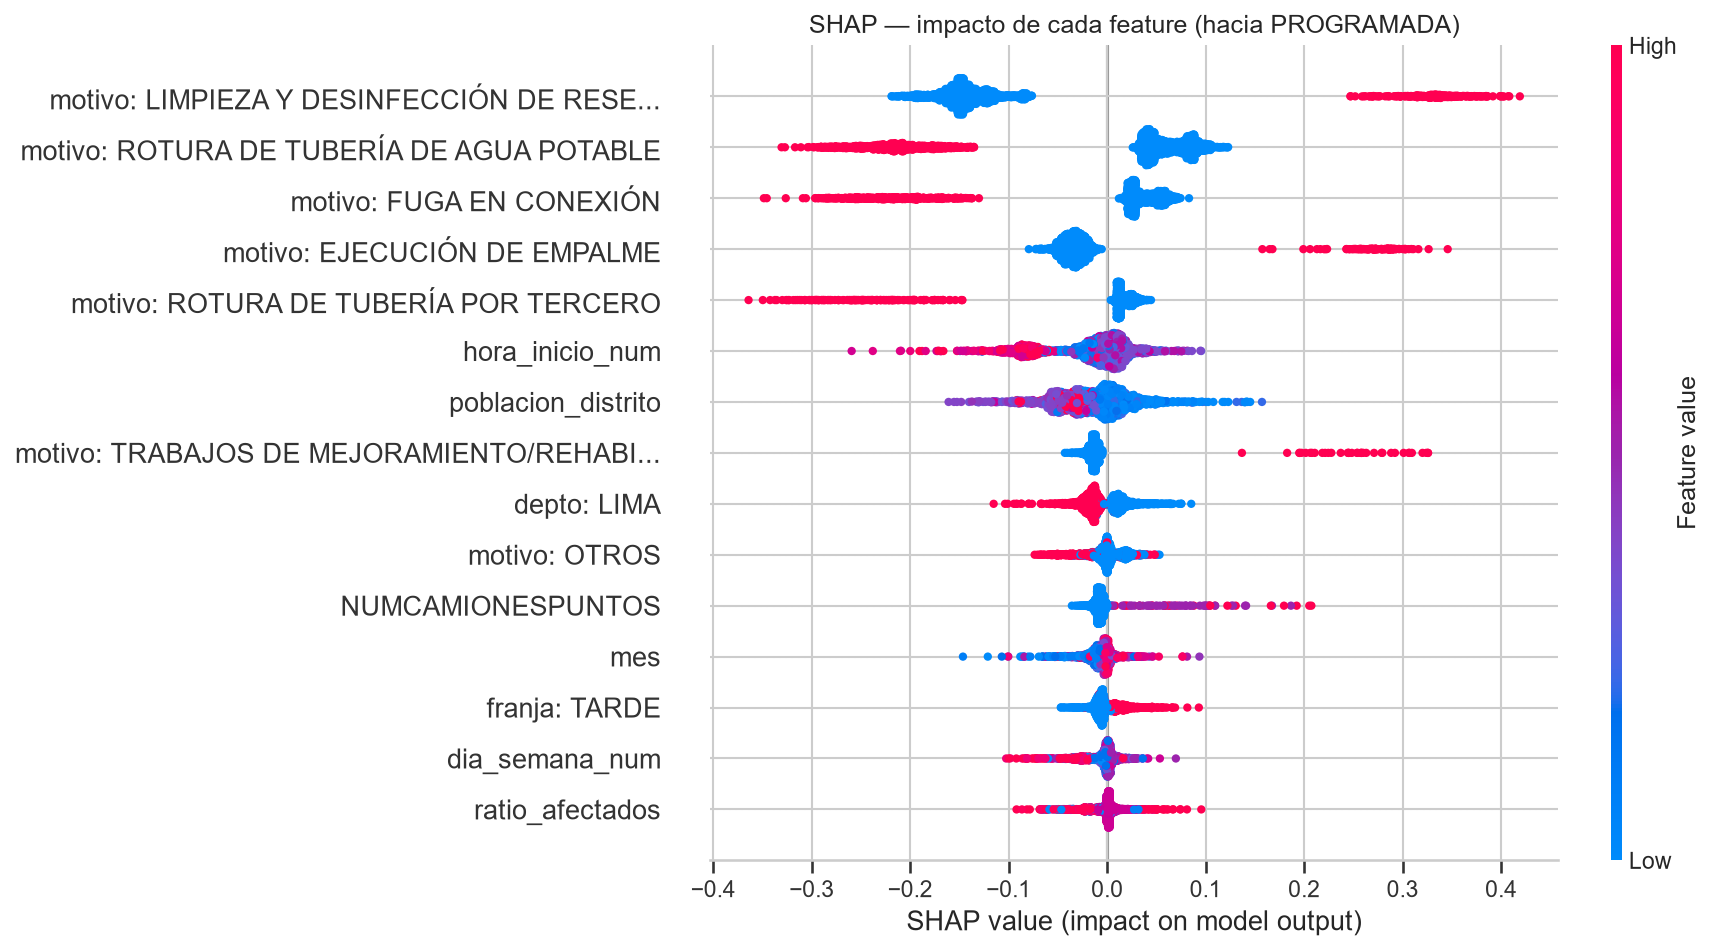
\includegraphics[width=0.92\textwidth]{figuras/shap_summary.png}
      \caption{Resumen SHAP del modelo ganador. Cada punto es un registro del test;
            el rojo indica valor alto de la variable y la posición horizontal, hacia dónde
            empuja la predicción.}
      \label{fig:shap}
\end{figure}

\begin{figure}[h]
      \centering
      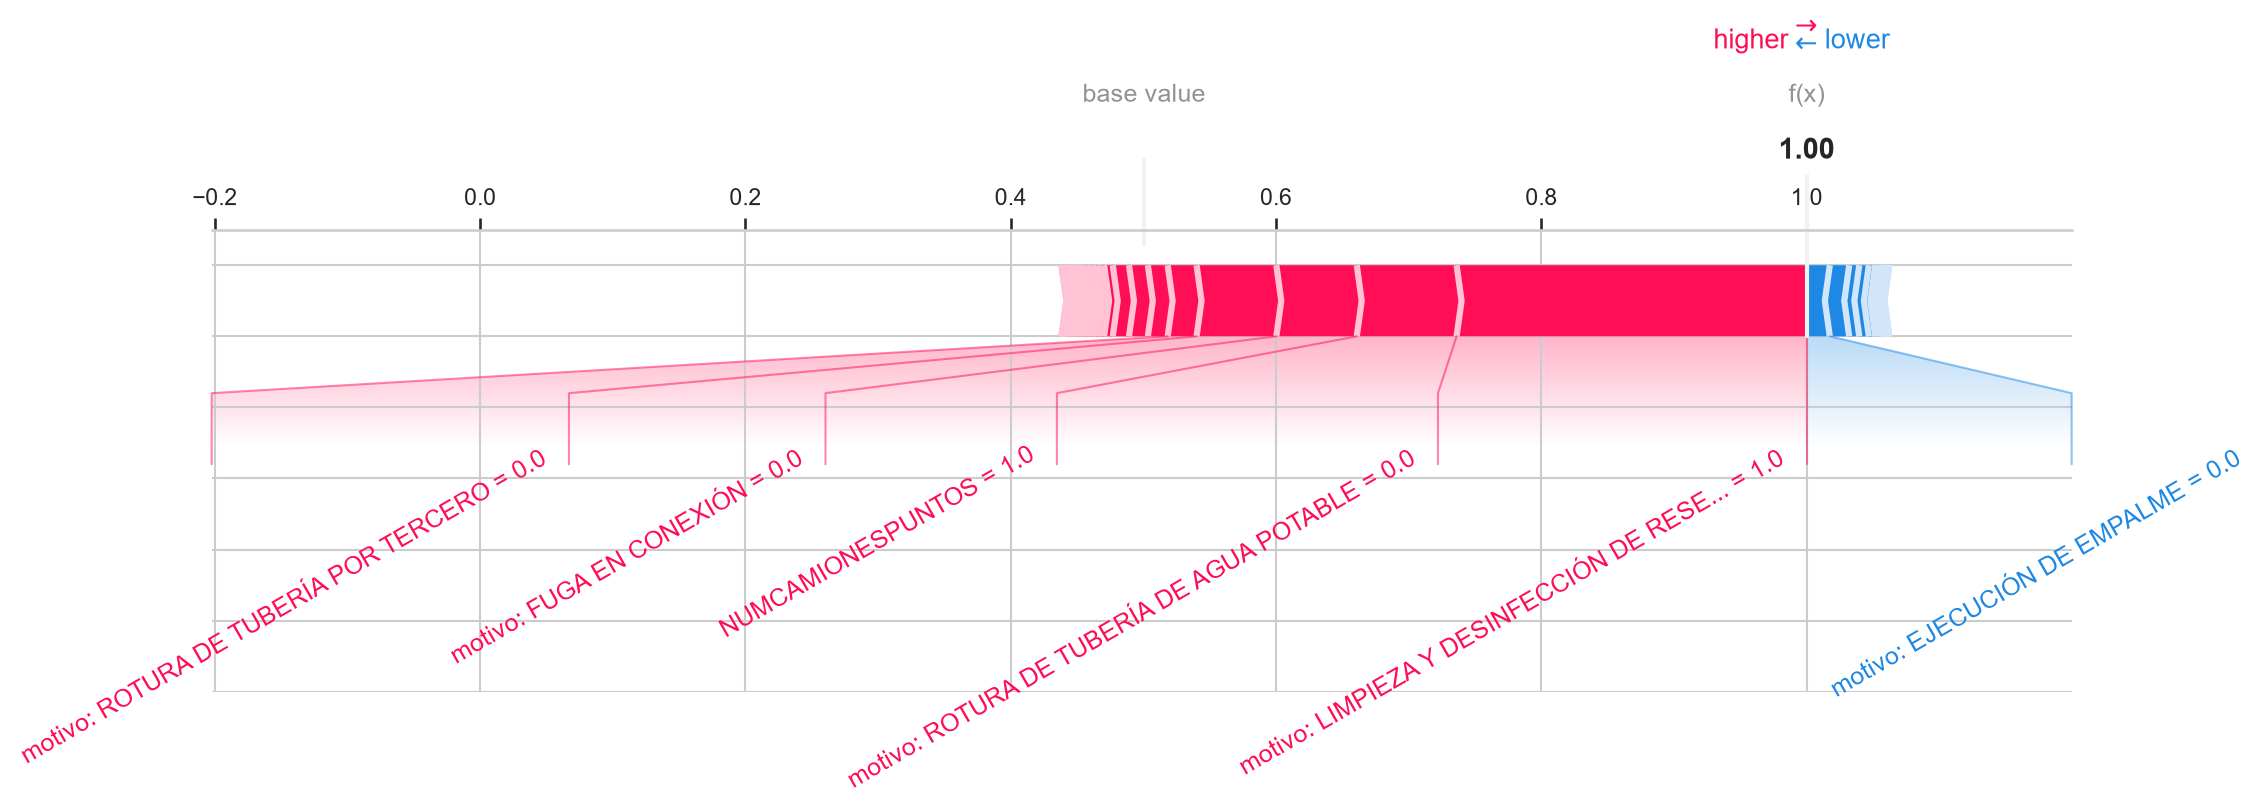
\includegraphics[width=\textwidth]{figuras/shap_force_caso.png}
      \caption{Force plot de un caso del test: corte de SEDAPAL en San Juan de
            Lurigancho por limpieza y desinfección de reservorio.}
      \label{fig:force}
\end{figure}

Para responder \guillemotleft ¿por qué el modelo predijo esto?\guillemotright{}
se explicó un caso concreto: un corte de SEDAPAL en San Juan de Lurigancho por
limpieza y desinfección de reservorio, clasificado PROGRAMADA con probabilidad
cercana a 1 (figura~\ref{fig:force}). El force plot muestra que tanto la
presencia del motivo de mantenimiento como la ausencia de los motivos de avería
empujan la predicción desde el valor base (la proporción histórica de
programadas) hacia arriba. LIME, aplicado al mismo caso con un modelo lineal
local, reproduce las mismas contribuciones, lo que da confianza en que la
explicación no es un artefacto del método.

\subsection{Clustering de distritos}

Sobre la matriz de 151 distritos se aplicó K-means con tres indicadores por
distrito: cortes por cada 10\,000 habitantes, duración mediana y porcentaje de
imprevistos. Las dos primeras tienen colas pesadas (asimetría de 2.3 y 2.6), así
que se transformaron con $\log(1+x)$ antes de estandarizar, para que un puñado
de distritos extremos no dominara la distancia euclídea.

El codo de inercia se produce en $k=4$, donde la ganancia marginal cae a la
mitad. La silueta es plana en todo el rango explorado (entre 0.27 y 0.34 para
$k$ de 2 a 8): su máximo en $k=8$ produciría grupos inaccionables y $k=2$ es
demasiado grueso, de modo que se eligió $k=4$ (silueta 0.310) por ser el punto
donde codo, silueta y legibilidad coinciden. DBSCAN, corrido como contraste,
marca 23 distritos atípicos que el panel muestra por separado.

\begin{table}[h]
      \centering
      \small
      \begin{tabular}{lcccc}
            \toprule
            \textbf{Perfil}                          & \textbf{Distritos} & \textbf{Cortes/10k hab} & \textbf{Dur.\ mediana (h)} & \textbf{\% imprevistas} \\
            \midrule
            Sed crónica (frecuente, breve, reactivo) & 57                 & 53.2                    & 5.1                        & 82.7                    \\
            Crítico (cortes largos e imprevistos)    & 24                 & 18.2                    & 17.8                       & 74.3                    \\
            Moderado (problema contenido)            & 53                 & 14.2                    & 6.3                        & 66.3                    \\
            Planificado (predominan programados)     & 17                 & 12.3                    & 11.3                       & 25.4                    \\
            \bottomrule
      \end{tabular}
      \caption{Perfil medio de los cuatro clusters ($k=4$, silueta 0.310).}
      \label{tab:clusters}
\end{table}

\subsection{Pronóstico semanal}
\label{sec:series}

La serie semanal de cortes a nivel país se pronosticó con tres métodos y un
backtest de corte temporal: entrenamiento hasta 12 semanas antes del final y
evaluación sobre esas 12 semanas, nunca con partición aleatoria. La media móvil
de 4 semanas obtiene un MAPE de 14.9\% (RMSE 38.5), ARIMA(2,1,1) un 15.1\%
(RMSE 39.4) y el suavizado exponencial de Holt-Winters queda atrás con 23.2\%.
El orden (2,1,1) salió de una búsqueda por mínimo AIC en la grilla
$p,q \in \{0,1,2\}$, $d \in \{0,1\}$.

Ante el empate técnico (menos de un punto de MAPE), la regla de desempate
declarada en el código prefiere el modelo estadístico: ARIMA entrega intervalos
de confianza fundamentados y reacciona a cambios de nivel, cosas que una media
móvil no puede ofrecer. Sobre la aceptabilidad del error: un MAPE de 15\% es
el piso de ruido de esta serie, pues ni el método ingenuo baja de ahí; la serie
tiene una componente aleatoria irreducible porque las roturas no se anticipan
una a una. El pronóstico final proyecta entre 200 y 216 cortes semanales para
las 8 semanas siguientes al fin de la ventana, con su banda de confianza del
95\% visible en el Panel 3.

% =====================================================================
\section{Narrativa: de la situación al impacto}

\textbf{Situación.} Un registro público de 45\,671 reportes que ninguna de las
partes usa de forma sistemática: SUNASS fiscaliza sin ranking objetivo de
distritos, las EPS reaccionan a las averías y los usuarios se enteran del corte
cuando abren el caño.

\textbf{Complicaciones y resoluciones.} El camino desde el CSV crudo hasta el
dashboard tuvo cinco obstáculos concretos, cada uno resuelto con una técnica del
curso:

\begin{itemize}
      \item \emph{Desbalance 76/24}: el accuracy engañaba (un modelo trivial ronda
            0.76 prediciendo siempre imprevisto). Se cambió la métrica objetivo a F1
            de la minoritaria y se aplicó \texttt{class\_weight='balanced'}, que
            subió el recall de PROGRAMADA de 0.885 a 0.918.
      \item \emph{Outliers extremos de duración}: distritos como Caspisapa y Pucacaca
            promedian 282 horas por corte cuando su mediana es de unas 8, y el máximo
            global llega a 8\,886 horas. Se reportan medianas y rango intercuartílico
            en lugar de medias, y el clustering usa $\log(1+x)$ para que esos
            extremos no distorsionen los centroides.
      \item \emph{50.5\% de nulos en conexiones afectadas}: la mitad de las EPS no
            reporta el dato. Se creó el indicador \texttt{reporta\_conexiones} para
            conservar esa señal y se imputó con la mediana calculada solo sobre el
            conjunto de entrenamiento, para no contaminar el test.
      \item \emph{Sospecha de fuga de información en el motivo}: se resolvió con un
            análisis de ablación (sin motivo: F1 0.753, AUC 0.923) y con el argumento
            temporal de que el motivo se conoce al reportar. Las variables que sí
            constituían fuga (duración, fecha de fin) se excluyeron desde el diseño.
      \item \emph{Bordes truncados de la serie}: las primeras y últimas semanas del
            registro tienen entre 1 y 8 eventos contra una mediana de 204, porque
            capturan el arranque del sistema y el corte de extracción. Con ellas
            dentro, el MAPE del backtest superaba el 260\%; recortando la ventana
            de análisis a junio de 2019 -- abril de 2024, baja al 15\%.
\end{itemize}

\textbf{Impacto.} Con estos resultados, cada actor tiene una decisión concreta
que hoy no puede tomar con el CSV crudo. SUNASS puede priorizar la fiscalización
en los 57 distritos del perfil \guillemotleft sed crónica\guillemotright{} y los
24 del perfil crítico, que concentran los cortes más frecuentes y los más largos.
Las EPS pueden activar el protocolo de contingencia (cisternas, comunicación)
cuando el clasificador marca un corte entrante como imprevisto, sabiendo que
cuando dice \guillemotleft programada\guillemotright{} acierta el 90.7\% de las
veces, y dimensionar las cuadrillas de la semana con un pronóstico que se
equivoca en promedio un 15\%, en una serie cuyo piso de ruido es ese mismo
orden. El módulo CRUD, por último, deja trazabilidad de cada consulta con marca
de tiempo, de modo que las predicciones usadas en una decisión quedan
registradas.

% =====================================================================
\section{Conclusiones}

El proyecto cumplió las cuatro metas que se fijó: dataset propio de 44\,043
registros construido por script desde una fuente peruana verificable, F1 de
0.912 en la clase minoritaria con seis modelos comparados, cuatro perfiles de
distrito con silueta 0.310 y un pronóstico a 8 semanas con MAPE de 15.1\%.
Más allá de las cifras, el hallazgo que ordena todo lo demás es que el tipo de
corte es altamente predecible en el momento del reporte, y que esa predicción
sobrevive incluso sin la variable de motivo; eso habilita automatizar la
respuesta de contingencia en lugar de depender de la clasificación manual de
cada EPS.

Quedan dos límites honestos. La silueta de 0.310 indica clusters útiles pero con
fronteras difusas, así que los perfiles deben leerse como herramienta de
priorización y no como categorías rígidas; y el pronóstico agregado a nivel país
no sustituye pronósticos por EPS, que serían el siguiente paso natural si SUNASS
quisiera operativizar la herramienta. Ambas extensiones caben sobre el mismo
pipeline sin rehacer la preparación de datos.

\paragraph{Entregables.} Repositorio con scripts, notebooks y dashboard:
\url{https://github.com/flyreh/datamining_final}. Dashboard desplegado en
Streamlit Cloud, accesible sin credenciales: \textit{(completar URL del deploy)}.
El CSV original y las instrucciones de reproducción están en el propio
repositorio (\texttt{descargas/} y \texttt{README.md}).

\end{document}
